\documentclass[00-GLMregslides.tex]{subfiles}
\begin{document}
	

%================================================ %
\begin{frame}[fragile]
\frametitle{Negative Binomial Regression with \texttt{R} }
\Large

% - R Data Analysis Examples: Negative Binomial Regression
\textbf{Introduction}
Negative binomial regression is for modeling count variables, usually for over-dispersed count outcome variables.

\end{frame}
%%	%================================================ %
%%	\begin{frame}[fragile]
%%	
%%	
%%	This page uses the following packages. Make sure that you can load them before trying to run the examples on this page. If you do not have a package installed, run: install.packages("packagename"), or if you see the version is out of date, run: update.packages().
%%	
%%	\begin{framed}
%%	
%%	
%%	
%%	
%%	
%%	
%%	
%%	
%%	\end{framed}
%%	


	
% Please note: The purpose of this page is to show how to use various data analysis commands. 
% It % does not cover all aspects of the research process which researchers are expected to do. In 
% particular, it does not cover data cleaning and checking, verification of assumptions, model 
% diagnostics or potential follow-up analyses.
%% \end{frame}
%================================================ %
\begin{frame}[fragile]
	\frametitle{Negative Binomial Regression with \texttt{R} }
	\Large
	
\textbf{Examples of negative binomial regression}
\begin{itemize}
\item \textbf{Example 1}  School administrators study the attendance behavior of high school juniors at two schools. \\ Predictors of the number of days of absence include the type of program in which the student is enrolled and a standardized test in math.

\item \textbf{Example 2}  A health-related researcher is studying the number of hospital visits in past 12 months by senior citizens in a community based on the characteristics of the individuals and the types of health plans under which each one is covered.
\end{itemize}
\end{frame}
%================================================ %
\begin{frame}[fragile]
	\frametitle{Negative Binomial Regression with \texttt{R} }
	\Large
	
\textbf{Description of the data}
Let's pursue Example 1 from above.
\begin{itemize}
\item We have attendance data on 314 high school juniors from two urban high schools in the file \textbf{negbin.csv }. 
\item The response variable of interest is days absent, \textbf{\textit{daysabs}}. 
\item The variable \textbf{\textit{math}} gives the standardized math score for each student. 
\item The variable \textbf{\textit{prog}} is a three-level nominal variable indicating the type of instructional program in which the student is enrolled.
\end{itemize}
\end{frame}
%================================================ %
%% \begin{frame}[fragile]
%%	\frametitle{Negative Binomial Regression with \texttt{R} }
%%	\Large
	
% Let's look at the data. It is always a good idea to start with descriptive statistics and plots.

%%	
%%	\begin{framed}
%%	
%%	
%%	
%%	
%%	
%%	
%%	
%%	\end{framed}

%% \end{frame}
%================================================ %
\begin{frame}[fragile]
\frametitle{Negative Binomial Regression with \texttt{R} }
\normalsize
\textbf{Exploratory Data Analysis}
\begin{framed}
\begin{verbatim}	
summary(dat)
        id         gender         math         daysabs     
  1001   :  1   female:160   Min.   : 1.0   Min.   : 0.00  
  1002   :  1   male  :154   1st Qu.:28.0   1st Qu.: 1.00  
  1003   :  1                Median :48.0   Median : 4.00  
  1004   :  1                Mean   :48.3   Mean   : 5.96  
  1005   :  1                3rd Qu.:70.0   3rd Qu.: 8.00  
  1006   :  1                Max.   :99.0   Max.   :35.00  
  (Other):308                                              
          prog    
  General   : 40  
  Academic  :167  
  Vocational:107  
\end{verbatim}	
\end{framed}

	
               
\end{frame}

\begin{frame}
\begin{figure}
\centering
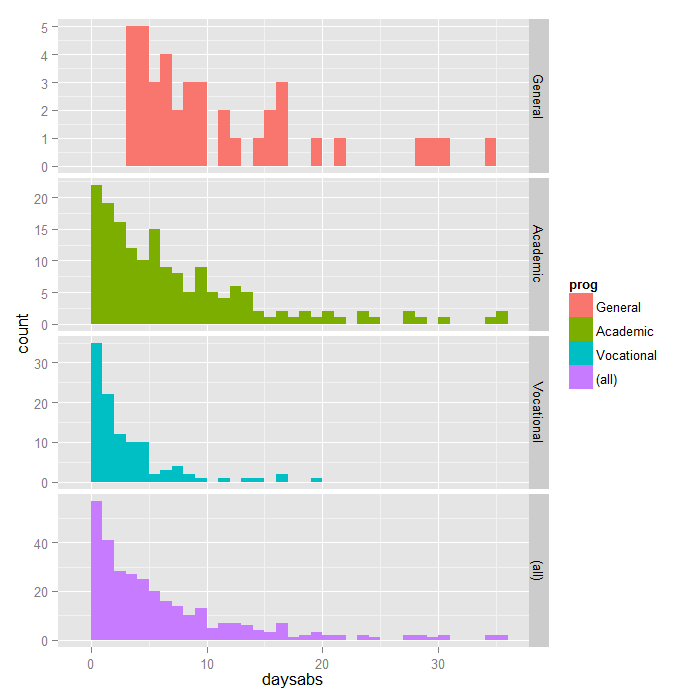
\includegraphics[width=0.99\linewidth]{negbin1}
%\caption{}
%\label{fig:negbin1}
\end{figure}

\end{frame}
%================================================ %
\begin{frame}[fragile]
	\frametitle{Negative Binomial Regression with \texttt{R} }
	\Large

\begin{verbatim}	
ggplot(dat, aes(daysabs, fill = prog)) + geom_histogram(binwidth = 1) + facet_grid(prog ~ 
., margins = TRUE, scales = "free")
\end{verbatim}
Histogram plots showing distribution of the data
Each variable has 314 valid observations and their distributions seem quite reasonable. The unconditional mean of our outcome variable is much lower than its variance.
\end{frame}

\end{document}
